恭喜你已经成功安装了ubuntu双系统,作为新手的你想来在刚刚的安装过程中一定是非常小心谨慎的,毕竟你也不想系统出现什么差错。在后续的工作中我们经常需要安装各种各样的安装包并对系统的环境进行配置,如果不小心配错了东西,重则系统可能无法正常工作(简称寄了)。这时候你就需要在启动页面进入“Ubuntu高级选项”对系统进行修复,或者直接重装系统。这是我们比较不愿意看到的情况,因此我们很有必要学习对系统的环境进行备份,这样即使环境配崩了也能恢复到配环境之前的状态,保留之前的工作。

\subsubsection{timeshift系统快照}

timeshift是linux上一款用于数据备份和恢复的软件,使用时会像相机一样给系统照个相。下面介绍一下timeshift的使用流程。

\textbf{安装timeshift}

\begin{tcode}
	sudo apt update
	sudo apt install timeshift
\end{tcode}

ubuntu也可以在软件中心直接搜索下载

\textbf{制作快照}

首先最好准备一个U盘,然后点击timeshift的图标启动,或者在终端输入

\begin{tcode}
	sudo timeshift-launcher
\end{tcode}

进入timeshift图形化操作界面,首先选择快照类型。RSYNC 是一种常见的文件同步协议,在 Timeshift 中用于增量式系统备份。备份时仅复制有改动的部分,因此通常比完整备份要小,创建速度更快。Btrfs 是一种支持快照等高级特性的文件系统。Timeshift 利用 Btrfs 的快照功能,可以创建系统的只读快照。这种类型的快照创建速度比 RSYNC 更快,占用的存储空间更小。但前提是,你的系统必须使用 Btrfs 文件系统。一般来说我们选择“RSYNC”。

备份位置最好选择在非系统硬盘或移动U盘,但要保证磁盘类型是ext4等linux类型。否则暂时选系统盘也行。选好盘后备份数据默认会保存在该硬盘下根目录下的 /timeshift 目录下。

备份时间有每月备份一次,每周备份一次、每日备份一次、每小时备份一次、每次开机备份一次,数字表示最多存几个快照,多了的话会删除最旧的那次快照。

“用户主目录”那栏根据自己需要的备份情况来选择,“筛选”那栏也是,可以选择添加所需目录或将其过滤。

\textbf{快照恢复}

如果系统损坏不大还可以正常使用,那么可以进入timeshift图形化界面,找到先前已经制作好的快照

\begin{figure}[H]
    \centering
    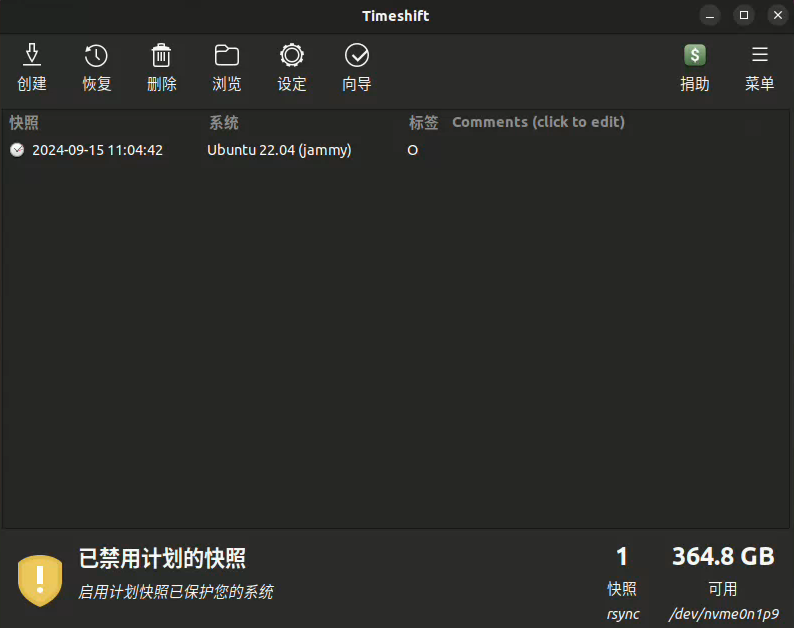
\includegraphics[width=0.7\textwidth]{restore1.png}
    \caption{timeshift图形化界面} % 图片标题
    \label{fig:restore1} % 图片标签,用于引用
\end{figure}

点击“恢复”,确认要恢复的目录后点击“下一步”即可进行恢复操作

\begin{figure}[H]
    \centering
    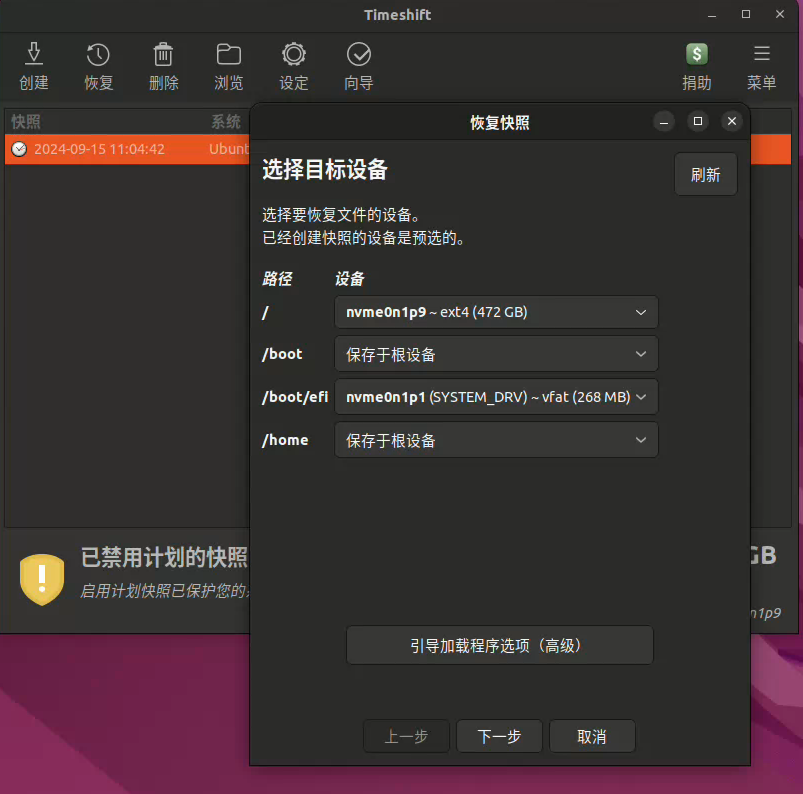
\includegraphics[width=0.7\textwidth]{restore2.png}
    \caption{timeshift快照恢复} % 图片标题
    \label{fig:restore2} % 图片标签,用于引用
\end{figure}

当然这个过程还可以通过命令行来完成:

备份快照

\begin{tcode}
	sudo timeshift --create --comments "快照名" --backup-device /dev/磁盘名
\end{tcode}

磁盘名可以通过 "fdisk -l" 或 "df -TH" 来查看

查看已存在的快照

\begin{tcode}
	sudo timeshift --list
\end{tcode}

选择上面已存在的其中一个快照进行恢复,如:快照'2024-07-01\_18-00-00'

\begin{tcode}
	sudo timeshift --restore --snapshot '2024-07-01_18-00-00' --skip-grub
\end{tcode}

如果已经无法加载图形化桌面,可以在开机时按“ctrl+alt+F1”(一般F1到F6都可以)进入tty终端,可以输入命令进行恢复。

如果连命令终端都进不去,只能通过启动盘再次进入安装ubuntu的页面,选择试用ubuntu,然后安装timeshift再进行恢复。

\subsubsection{系统镜像备份}

linux秉承着一切皆文件的思想,系统备份就相当于把整个根目录所有文件打包压缩保存。

\textbf{镜像制作}

备份前先切换到root用户,避免权限问题,然后切换到根目录,输入

\begin{tcode}
	tar -cvpzf /media/Disk/myDisk/ubuntu_backup@`date +%Y-%m+%d`.tar.gz --exclude=/proc --exclude=/tmp --exclude=/boot --exclude=/home --exclude=/lost+found --exclude=/media --exclude=/mnt --exclude=/run /
\end{tcode}

下面解释一下上面这条命令:tar就是一个打包命令,

\begin{tcode}
	/media/Disk/myDisk/ubuntu_backup@`date +%Y-%m+%d`.tar.gz
\end{tcode}

这个是备份文档的存放路径,myDisk表示你的移动硬盘名字,挂载在/media/Disk目录下,

\begin{tcode}
	ubuntu_backup@date +%Y-%m+%d.tar.gz
\end{tcode}

这是备份文件的名字,这里用了一个shell命令

\begin{tcode}
	date +%Y-%m+%d
\end{tcode}

用于记录备份时间。接下来看看–exclude参数中的内容。

假设现在ubuntu中有四个分区:/、/home、/boot、swap,其中/home、/boot两个分区出问题的概率很小,而且变动也不会太频繁,因此在定期备份时可以减小对这两个分区的备份频率。一般系统坏了都是/分区的问题,/home没什么关系。再来看看其他排除的目录:

/proc:一个虚拟文件系统,系统运行的每一个进程都会自动在这个目录下面创建一个进程目录。既然是系统自动创建,也就没必要备份的必要了。

/tmp:一个临时文件夹,系统的一些临时文件会放在这里。

/lost+found:系统发生错误时(比如非法关机),可以在这里找回一些丢失文件。

/media:多媒体挂载点,像u盘、移动硬盘、windons分区等都会自动挂载到这个目录下。

/mnt:临时挂载点,你可以自己挂载一些文件系统到这里。

/run:系统从启动以来产生的一些信息文件。

另外,有可能备份到最后系统会提示"tar: 由于前次错误,将以上次的错误状态退出",这个警告可以忽略,没什么影响的。

\textbf{镜像恢复}

这里有两种还原方式:

\begin{enumerate}
    \item 直接操作
    
    如果你系统出问题了,但是还可以进入终端,那就可以直接解压备份文件进行还原。切换到root,并且换到/根目录,打开终端,输入
    
    \begin{tcode}
        tar -xvpzf /media/Disk/myDisk/ubuntu_boot_backup@2016-6-6.tar.gz -C /
    \end{tcode}

    \item 使用启动盘还原
    
    如果你连系统都不能登录了,就要使用U盘启动盘进行还原了。依旧是先进入试用ubuntu界面,切换到root,打开终端,输入

    \begin{tcode}
        mkdir /mnt/sys
        mount /dev/sdaX /mnt/sys
        tar -xvpzf /media/myDisk/ubuntu_boot_backup@2016-6-6.tar.gz -C /mnt/sys
    \end{tcode}

    注意先创建一个临时目录用于挂载你的/根目录分区,sdaX代表你的/根目录分区,如果不知道就用fdisk -l查看一下,另外如果你的移动硬盘没有被自动挂载,你也需要手动创建一个临时目录进行挂载。

    因为 tar还原是只会覆盖相同的文件,但是这种方法只是恢复备份时的文件,就是说如果某些文件丢失或损坏了,这样可以恢复修复这些文件,但不能删除自备份到恢复前这期间所生成的其它文件,说白了就是假如你备份系统时有1234这四个文件,如果三天后,由于某些原因变成了1234’5(4改变了),你恢复后,就会变成12345,其中4’恢复成备份时的文件,5保留。
\end{enumerate}

